\documentclass[11pt]{article}
    \usepackage{caption}
    \usepackage{graphicx}
    \usepackage{mathtools}
    \usepackage{bookmark}
    \graphicspath{ {img/} }
    \setlength{\parindent}{0pt}
    \DeclareCaptionType{equ}[][]
    \usepackage[svgnames]{xcolor}
    
    \newcommand*{\plogo}{\fbox{$\mathcal{BM}$}}
    
    \usepackage{PTSerif}
    
    \begin{document} 
        
    \begin{titlepage}
    
        \raggedleft
        
        \vspace*{\baselineskip}
        
        {\Large Bryan Melanson}
        
        \vspace*{0.167\textheight}
        
        \textbf{\LARGE How to Not Fail}\\[\baselineskip]
        
        {\textcolor{Red}{\Huge Probability \& Random Processes}}\\[\baselineskip]
        
        {\Large \textit{While never going to class}}
        
        \vfill
        
        {\large Computer Engineering 2020 ~~\plogo}
        
        \vspace*{3\baselineskip}
    
    \end{titlepage}

    \pagebreak
    
%%%%%%%%%%%%%%%%%%%%%%%%%%%%%%%%%%%%%%%%%%%%%%%%%
    \pdfbookmark[section]{\contentsname}{toc}
    
    \tableofcontents

%%%%%%%%%%%%%%%%%%%%%%%%%%%%%%%%%%%%%%%%%%%%%%%%%
    \pagebreak
    \section{Descriptive Statistics}

    \subsection{Statistics}
    Statistics are the summarization of a set of data that has been collected, which demonstrates random variation. \textit{Extracting meaning from data.}

    \subsection{Inferential Statistics}
    Making inferences about a situation based on data, such as forecasting. \\
    Descriptive statistics can be the basis for inferences.

    \subsection{Representative Values}
    \begin{enumerate}
        \item{Mean} 
        \item{Median}
        \item{Mode}
        \item{Range \textit{- [Min, Max]}}
        \item{Variance \textit{- Average of deviation squared from the mean}}
        \item{Standard Deviation \textit{- Measure of average absolute deviation}}
        \item{Skewness \textit{- Measure of the shape of the distribution funciton}}
        \item{Quantiles \textit{- Generalization of the median to percentiles}}
    \end{enumerate}
    \subsection{Observational vs. Experimental Data}
    Experimental involves manipulation objects to determine cause and effect in data. Observational refers to naturally occurring events.
    \pagebreak

%%%%%%%%%%%%%%%%%%%%%%%%%%%%%%%%%%%%%%%%%%%%%%%%%

    \section{Basic Probability}
    \subsection{Probability Calculus}
    Probability events have a total probability between zero and one.
        \begin{equ}[!ht]
            \begin{equation}
              Pr[An Event] = 1
            \end{equation}
          \caption{An event which is sure to happen}
        \end{equ} 

The definition of probability for how often an event is observed can be related to the number of repetiions of the experiment. \\


\begin{equ}[!ht]
    \begin{equation}
      Pr[Heads] =  \frac{\textrm{number } k \textrm{ of Heads in }N \textrm{ coin tosses}}{\textrm{ coin tosses}}
    \end{equation}
  \caption{Counting the probability of heads in a set of coin tosses}
\end{equ} 

The larger the number of repetiions, the higher accuracy with which we can predict the likelihood of an event happening.

\subsection{Probability Model}

\subsubsection{Events}
Events are elements in the set of possible outcomes in an experiment.

\subsubsection{Sample Space}
The set of all possible outcomes for an experiment.

\begin{equ}[!ht]
    \begin{equation}
      S = \{1,2,3,4,5,6\}
    \end{equation}
  \caption{The sample space for a dice roll}
\end{equ} 

\begin{equ}[!ht]
    \begin{equation}
      A_1 = \{1\}, A_2 = \{1,2,5\}
    \end{equation}
  \caption{Subsets containing events in the sample space}
\end{equ} 

The complement of a subset $A^C$ is the subset of all other events in the sample space which are not contained in $A$.

\subsection{Event Algebra}

\subsubsection{Or}
The combination of two or more sets.\\

For $A = \{1,2,5\}$ and $B = \{3, 4\}$, $A_1 + A_2 = \{1, 2, 3, 4, 5\}$

\subsubsection{And}
The set of events which occur in two or more sets.\\

For $A = \{1,2,3, 5\}$ and $B = \{3, 4\}$, $A_1A_2 = \{3\}$

\subsubsection*{Axioms}
\begin{enumerate}
    \item{Mutual exclusion: } $AA^c = 0$
\item{Inclusion: } $AS = A$
\item{Double complement: }$(A^C)^C = A$
\item{Commutation: } $A_1 + A_2 = A_2 + A_1$
\item{Associativity: } $A_1 + (A_2 + A_3) = (A_1 + A_2) + A_3$ 
\item{Distributivity: } $A_1 (A_2 + A_3) = A_1A_2 + A_1A_3$
\item{DeMorgan’s Law: } $(A_1A_2)^c = (A_1)^C + (A_2)^C$
\end{enumerate}

\subsection{Probability of Events}

\subsubsection*{Axioms}
\begin{enumerate}
    \item{For any event $A$: $Pr[A] \geq 0$} 
    \item{$Pr[S] = 1$}
    \item{If $A$ and $B$ are \textbf{Mutually Exclusive} then } $Pr[A + B] = Pr[A] + Pr[B]$
    \begin{center}
        \textbf{Mutual Exclusivity} refers to the fact that $A$ and $B$ will never occur simultaneously, ie $AB = 0$.
    \end{center}
\item{Axiom 3 can be extended: } $Pr[A_1 + A_2 + ... ] = Pr[A_1] + Pr[A_2] + ...$
\end{enumerate}

\subsubsection{Non-Mutually Exclusive}
In cases where $A$ and $B$ can occur in the same set, Axiom 3 will not apply. \\
This is due to the fact that in overlapping events, the same area of probability will be counted twice, though it has no statistical importance.

\begin{equ}[!ht]
    \begin{equation}
      Pr[A_1 + A_2] = Pr[A_1] + Pr[A_2] - Pr[A_1A_2]
    \end{equation}
  \caption{Non mutually exclusive OR}
\end{equ} 

\subsubsection{Complement of an event}
From expanding on these axioms, it can be seen that the complement of an event has a probability related to subtraction of itself from the sample space probability. If the chance of the event happening is known, the chance of an event not happening is found by subtracting this from absolute certainty.

\begin{equ}[!ht]
    \begin{equation}
      Pr[A^c] = 1 - Pr[A]
    \end{equation}
  \caption{The complement of a set versus the whole}
\end{equ} 

\subsubsection{Statistical Independence}

\textit{Two events $A$ and $B$ are said to be statiscally independent if}

\begin{equ}[!ht]
    \begin{equation}
      Pr[AB] = Pr[A]Pr[B]
    \end{equation}
  \caption{Statistical independence}
\end{equ} 

This refers to the fact that statistical data will happen independent of the preceding events. If you flip a coin, the probability of the next coin will be the same. If you take items from a bin, the probability of the next item being picked will go up, and is therefore dependent.
\subsection{Repeated Independent Trials}

From the rule of statistical independence, we can process repeated trials:
\subsubsection*{Coin Flips}
$Pr[H] = p$ \\

$Pr[T] = Pr[H^c] = 1 - p = q$ \\

$Pr[HHH] = ppp = p^3$ \\

$Pr[HTH] = pqp = p^2q$ \\


Knowing that the probability of either event is 0.5, we can take the list of possible outcomes and calculate the probability. \\


$Pr[\textit{At least two heads}] = Pr[HHH] + Pr[HHT] + Pr[HTH] + Pr[THH]$ \\ 

$ = ppp + ppq + pqp + qpp $ \\

$ = (0.5)^3 + (0.5)^2*(0.5) + (0.5)^2*(0.5) + (0.5)*(0.5)^2$ \\

$ = 0.5 $ \\

$Pr[\textit{No heads}] = Pr[TTT] = q^3 = 0.125$

\subsubsection{Sampling With Replacement}

In this case, we consider an event where an event occurring does not subtract from a finite amount of events, ie a coin flip. In the case of heads or tails, there aren't one less heads or tails. So it is as if we replace the event in our sample space.

\subsubsection{Sampling Without Replacement}

Finite amounts of events that can be subtracted from the whole. If this event happens, it won't happen again, as if we have taken our card from a deck of cards and not placed it back in the deck.

\subsubsection{Order of Outcomes When Sampling Without Replacement}

Cases when its important what order events occur in. Did we draw the Ace of Spades within the first 3 draws? The number of each event is not important. \\

\textbf{K-Tuples} \\

When a trial is repeated $k$ times, we form a sample space of outcomes made up of $k$ number of events. \\


\subsubsection{The Rule of Product}

How many possibilities are there for the formation of $k$-tuples, if there are $N_i$ choices for the $i$th  element? \\

\begin{equ}[!ht]
    \begin{equation}
        N_1 * N_2 * ... N_k
    \end{equation}
  \caption{The Rule of Product}
\end{equ} 

By this rule, the number of possibilities when rolling a dice, then flipping a coin, will be $6 * 2$. In the case where same number of outcomes are possible with each experiment, the number of $k$-tuples is $N^k$, or $2^k$ in the case of repeated coin tosses. \\


\subsubsection{Permutations or Unordered Outcomes}

We no longer care in what order outcomes occur, we are only concerned with the number of outcomes of a certain sort across all trials. \\

This involves the number of ways we can choose $k$ objects in $N$ choices.

\subsubsection*{Permutations Without Replacement}

\begin{itemize}
    \item Experiments with two or more possible outcomes
    \item These trials can be repeated independently for $N$ times
    \item For each $k$th trial the outcome from the previous is removed
    \item Probabilities change for each consecutive trial
\end{itemize}

The resulting set is ordered, but as mentioned before, we only care about the number of possible permutations from these elements. \\

The number of possible sets is $N!$ or $N * (N-1) * (N-2) * ... 2 * 1$ \\

\textbf{Example} - The 13 cards of a suit in a deck of cards can be laid out in $13!$ or $6227020800$ different ordered sequences. \\

If you want just $k$ draws from $N$ possible ways to draw the object, the number of sets will instead be from $N$ to $(N-k+1)$ \\

Consider this problem - Lisa has 13 different ornaments and wants to put 4 ornaments on her mantle. In how many ways is this possible? \\


Using the product rule, Lisa has 13 choices for which ornament to put in the first position, 12 for the second position, 11 for the third position, and 10 for the fourth position. So the total number of choices she has is $13 * 12 * 11 * 10$. Using the factorial notation, the total number of choices is $\frac{13!}{9!}$. \\

From this example, we can see that if we have $N$ objects and want to arrange $k$ of them in a row, there are $\frac{N!}{(N-k)!}$ ways to do this. \\

\textbf{The notation for permutations is $P^{13}_3$}
\subsubsection{Combinations or Non-Unique Outcomes}

A \textit{combination} is a way of choosing elements from a set in which order does not matter. \\


Consider the following example: Lisa has $13$ different ornaments and she wants to give $3$ ornaments to her mom as a birthday gift (the order of the gifts does not matter). How many ways can she do this? \\

We can think of Lisa giving her mom a first ornament, a second ornament, a third ornament, etc. This can be done in $P^{13}_3$ ways. However, Lisa's mom is receiving all three ornaments at once, so the order Lisa decides on the ornaments does not matter. 
There are $3!$ reorderings of the chosen ornaments, implying the total number of ways for Lisa to give her mom an unordered set of $5$ ornaments is $\frac{13!}{10!3!}$. \\

\begin{equ}[!ht]
    \begin{equation}
        \frac{N!}{N!(N!-k!)}
    \end{equation}
  \caption{Rule of Combinations or Unordered Permutations}
\end{equ} 

\textbf{The notation for combinations is $C^{N}_k$ = ${N}\choose{k}$} \\

The number of ways to choose $k$ objects \textit{in any order} from a set of $N$ objects.

\subsection{Conditional Probability}

A \textbf{conditional probability} is a probability that a certain event will occur given some knowledge about the outcome or some other event. \\

$P[A|B]$ is a conditional probability, it is read as "Probability of A given B". \\

\begin{equ}[!ht]
    \begin{equation}
        Pr[A|B] = \frac{Pr[AB]}{Pr[B]}
    \end{equation}
  \caption{Rule of Conditional Probability}
\end{equ} 

A simple example - A fair 12-sided die is rolled. What is the probability that the roll is a 3 given that the roll is odd? \\

This is $Pr[3|Odd]$ or $\frac{Pr[3]Pr[Odd]}{Pr[Odd]}$ \\

Because $B$ has already happened, the intersection of $B$ and $A$ can have the $B$ probability removed, because it is statistically redundant. \\

\begin{equ}[!ht]
    \begin{equation}
        Pr[A|B] = \frac{Pr[AB]}{Pr[B]} = \frac{Pr[B]Pr[A]}{Pr[A]} = Pr[B]
    \end{equation}
  \caption{Conditional Probability if statiscally independent}
\end{equ} 

\subsubsection{Bayes Theorem}

When attempting to compute the conditional probability of two events, when only one event is known, the Bayes Theorem allows for a workaround. \\

\textit{Consider $H$ to be Hypothesis, and $E$ to be Evidence}

\begin{equ}[!ht]
    \begin{equation}
        Pr[H|E] = \frac{Pr[E|H] Pr[H]}{Pr[E]}
    \end{equation}
  \caption{Bayes Theorem}
\end{equ} 

We can expand the equation in the numerator to demonstrate fully: \\

$Pr[E|H]Pr[H] = \frac{Pr[EH]}{Pr[H]}*Pr[H] = Pr[EH] = Pr[HE]$ \\ 

Therefore, $Pr[H|E]$ or $\frac{Pr[HE]}{Pr[E]}$ can be found from $Pr[E|H]$ and vice versa. 

\subsubsection{Total Probability}

If $A_1, A_2$, and $A_3$ form a partition of the sample space, for each $A_i$

\begin{equ}[!ht]
    \begin{equation}
        Pr[A_i|B] = \frac{Pr[B|A_i] Pr[A_i]}{Pr[B]}, i = 1,2,3
    \end{equation}
  \caption{Total Probability}
\end{equ} 

Knowing this, $Pr[B]$ can be found from $Pr[B|A_1] + Pr[B|A_2] + Pr[B|A_3]$

\begin{equ}[!ht]
    \begin{equation}
        Pr[A_i|B] = \frac{Pr[B|A_i] Pr[A_i]}{Pr[B|A_1] + Pr[B|A_2] + Pr[B|A_3]}, i = 1,2,3
    \end{equation}
  \caption{Bayes General Rule}
\end{equ} 

\begin{equ}[!ht]
    \begin{equation}
        Pr[B] = Pr[B|A_1] + Pr[B|A_2] + Pr[B|A_3]
    \end{equation}
  \caption{Total Probability, when $A_1$, $A_2$, $A_3$ form a partition}
\end{equ}

\pagebreak

%%%%%%%%%%%%%%%%%%%%%%%%%%%%%%%%%%%%%%%%%%%%%%%%%

\section{Random Variables}
Random variables deal with a function $X$ which maps a number $x$ from the sample space $S$. The number can be placed on the real number line, and a probability assigned to it based on its random occurrence.
\subsection{Discrete Probability Distributions}
Discrete random variables involve events with a discrete set of values.
\subsubsection{Probability Mass Function}
The \textit{Probability Mass Function}, or \textbf{PMF} $f_k [k]$ is a plotting of the probability of all events associated with a random variable $K$. The sum of all amplitudes of the graph, $\sum f_k [k]$ will be 1.
\begin{figure}[h]
    \centering
    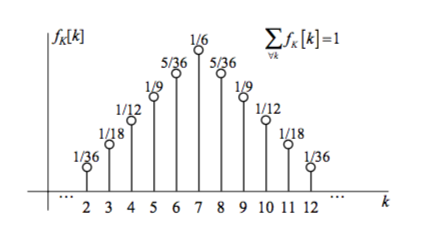
\includegraphics[width=\textwidth]{pmf}
    \caption{Probability Mass Function}
    \label{fig:pmf}
\end{figure}

For a given value $k$, the probability of this value is $f_k[k] = Pr[K = k]$.
\subsubsection{Bernoulli Random Variable}
A Bernoulli RV is a discrete variable which will only produce values of $1$ and $0$. Therefore, the likelhood of one will be $p$ and the other will be $1-p$.
\subsubsection{Binomial Random Variable}
The Bernoulli concept can be extended with combinatorics, for example in the base of binary transmission error. When detecting the error in the first $n$-bits of a $k$-bit transmission, $f_K[k] =$ $n\choose{k}$ $p^k(1-p)^{(n-k)}$. 
\\ 

As shown in earlier sections, there are $n\choose{k}$ possible variations of $k$ bits in an $n$-bit long transmission. If our likelihood of non-error bits is $p$, and error is $(1-p)$, the above will be intuitively correct.
\subsubsection{Geometric Random Variable}
Geometric RVs concern a wait for an event to happen. Should the expected event be given $p$ probability, there will be $k$ consecutive $(1-p)$ events before the $p$ occurs. Therefore, as seen in the graph below, the event occuring at the second transmission will be $(1-p)^2p$. 
\begin{figure}[h]
    \centering
    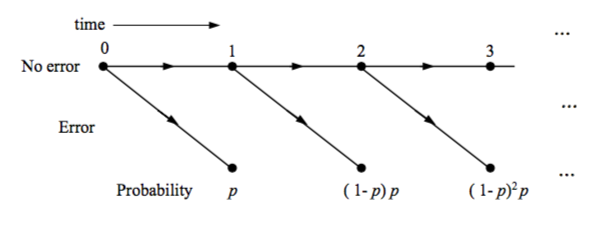
\includegraphics[width=\textwidth]{geo1}
    \caption{Geometric Random Variable}
    \label{fig:geo1}
\end{figure}

\begin{equ}[!ht]
    \begin{equation}
        f_K[k] = p(1-p)^k
    \end{equation}
  \caption{Geometric Random Variable PMF (0 $\leq$ k $<$ $\infty$)}
\end{equ} 

\subsubsection{Poisson Random Variable}
For a situtation where revents occur randomly at a given rate $\lambda$ over a certain time interval $t$, the probability of $k$ events happening within this time frame has been experimentally verified with $\lambda t$ representing the average.
 
\begin{equ}[!ht]
    \begin{equation}
        f_K[k] = \frac{(\lambda t)}{k!}e^{-a}
    \end{equation}
  \caption{Poisson Random Variable PMF}
\end{equ} 

\begin{figure}[h]
    \centering
    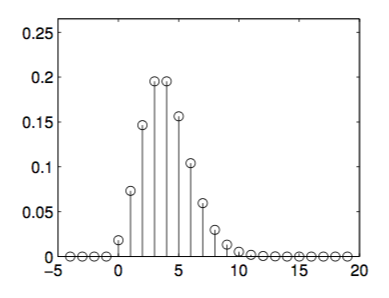
\includegraphics[width=\textwidth]{poisson}
    \caption{Poisson Distribution}
    \label{fig:poisson}
\end{figure}

Note that for finding the probability of an event occurring after time $t$, the probability becomes $Pr[0] + Pr[1] + Pr[2] ... + Pr[t]$.

\subsubsection{Uniform Random Variable}

When all events are equally likely, the probability of each can be found easily from the uniform random variable PMF.

\begin{equ}[!ht]
    \begin{equation}
        f_K[k] = \frac{1}{n - m + 1}
    \end{equation}
  \caption{Uniform Distribution}
\end{equ} 

\begin{figure}[h]
    \centering
    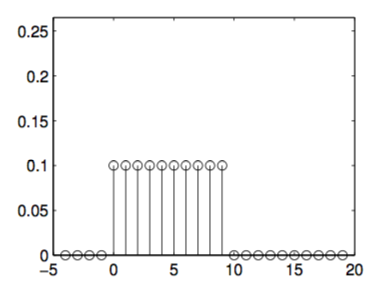
\includegraphics[width=\textwidth]{uniform}
    \caption{Uniform Distribution}
    \label{fig:uniform}
\end{figure}

\subsection{Continuous RVs and Their Distributions}

For values which can take on a continuum of values, such as voltage, velocity, and mass, new tools are used to analyze their probability. The probability of these events is determined using the \textit{Cumulative Distribution Function} or \textbf{CDF}, which is written as $F_X(x) = Pr[X \leq x]$. \\

By this notation we can see that by following the graph from left to right, the probability of the event occuring to the \textbf{left} of value $x$ will be found by the amplitude of the CDF at that value. Therefore, as $x \rightarrow \infty$, $F_x \rightarrow 1$. \\


\begin{figure}[h]
    \centering
    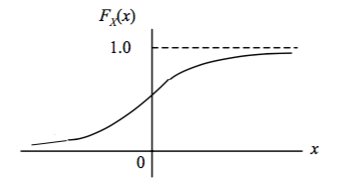
\includegraphics[width=\textwidth]{cdf}
    \caption{Continuous Density Function}
    \label{fig:cdf}
\end{figure}

When finding the probability of a value occurring between points $a$ and $b$, their CDF values can be used. \\


\begin{equ}[!ht]
    \begin{equation}
        Pr[a < X \leq b] = F_X(b) - F_x(a)
    \end{equation}
  \caption{CDF Probability Within a Range (b $>$ a)}
\end{equ} 

The \textit{Probability Density Function} or \textbf{PDF} is a derivative of the CDF that can also be used to find this probability:

\begin{figure}[h]
    \centering
    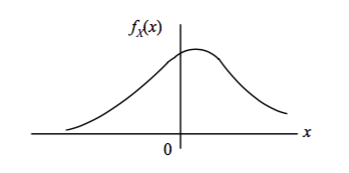
\includegraphics[width=\textwidth]{pdf1}
    \caption{Probability Density Function}
    \label{fig:pdf}
\end{figure}

\begin{equ}[!ht]
    \begin{equation}
        Pr[a < X \leq b] = \int_{b}^{a}f_X(x)dx 
    \end{equation}
  \caption{CDF Probability Within a Range (b $>$ a) From Integration}
\end{equ}  

This can be seen to be similar to the Probability Mass Function, as it will integrate over its full range to 1 -  $\int_{\infty}^{\infty}f_X(x)dx = 1$ \\

To use the PDF to find the probability of a number $a + \Delta x$, we can multiply the PDF value at this point by the increment value to find the probability.

\begin{equ}[!ht]
    \begin{equation}
        Pr[a < X \leq a + \Delta x] = f_X(a) \cdot \Delta x
    \end{equation}
  \caption{PDF Probability Within a Range ($a$ $<$ $a + \Delta x$)}
\end{equ} 

Integrating over a range ($a, b$) will also produce $Pr[a < x \leq b]$ from the PDF.

\subsection{Common Continuous RVs}

\subsubsection{Exponential Random Value}

An extension of the Geometric Random Variable to the continuous realm, this represents a continuous graph of wait times where again $\lambda$ represents the rate of arrival for an event as in Poisson RVs.\\

Its PDF follows $f_X(x) = \lambda e^{-\lambda x}$

\subsubsection{Gaussian RV}

The Gaussian or "normal" random variable arises naturally in numerous cases. It can be defined by its mean, $\mu$, which will be the center of its bell shape, and its standard deviation $\sigma$, which denotes the value in each direction it will pass before reaching $60.7\%$ of its peak value. \\

\begin{equ}[!ht]
    \begin{equation}
        f_X(x) = \frac{1}{\sqrt{2\pi \sigma ^2}} e^{-(x-\mu)^2/2\sigma ^2}
    \end{equation}
  \caption{The Gaussian PDF}
\end{equ} 


\begin{figure}[h]
    \centering
    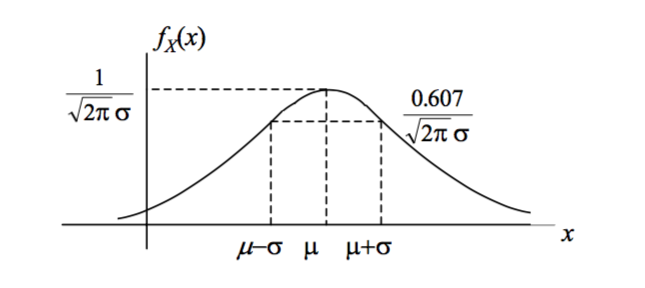
\includegraphics[width=\textwidth]{gauss}
    \caption{Gaussian Random Variable}
    \label{fig:gauss}
\end{figure}

The square of the standard deviation, $\sigma ^2$ is known as the variance, and is a measure of the total width of the bell between these points.\\



The standard form of the PDF, centered at $0$ with a $\sigma ^2$ $=1$ can be used to express $Pr[X \leq x]$:

\begin{equ}[!ht]
    \begin{equation}
        \Phi(x) = \frac{1}{\sqrt{2\pi}} \int_{\infty}^{x}e^{-x^2/2}
    \end{equation}
  \caption{The Standard Gaussian Function}
\end{equ} 

\begin{center}
    $F_X(x) = Pr[X \leq x] = \Phi (\frac{x - \mu}{\sigma})$
\end{center}

And as with any other CDF, $Pr[a < x \leq b] = F_X(b) - F_x(a)$ \\


\begin{figure}[h]
    \centering
    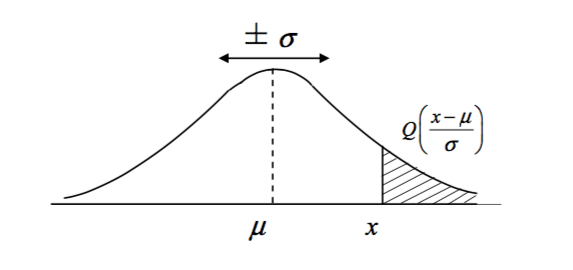
\includegraphics[width=\textwidth]{q1}
    \caption{Probability Using Q ($x$ $>$ $\mu$)}
    \label{fig:q1}
\end{figure}

These $\Phi$ values, which can be used as a CDF, as with other standard Gaussian values, can be found by table. 

\subsubsection{Gaussian Q Values}

In cases where the probablity of values at either tail of a Gaussian is required, such as $Pr[a < x \leq \infty]$, it is common to use $Q$ functions.

\begin{equ}[!ht]
    \begin{equation}
        Q(x) = 1 - \Phi(x)
    \end{equation}
  \caption{The Gaussian Q Function}
\end{equ} 

When a value $x$ is sought which is less than $\mu$, the argument of the $Q$ function will be negative, and define the left tail of the CDF. 

\begin{equ}[!ht]
    \begin{equation}
        Pr[X < x] = Q(\frac{x - \mu}{\sigma})
    \end{equation}
  \caption{The Gaussian Q Function}
\end{equ}

\begin{equ}[!ht]
    \begin{equation}
        Pr[X > x] = Q(\frac{- x + \mu}{\sigma})
    \end{equation}
  \caption{The Gaussian Q Function with Negative Argument}
\end{equ} 

\begin{center}
    $Pr[a \leq x \leq b] = Q(\frac{b-\mu}{\sigma}) - Q(\frac{a-\mu}{\sigma})$
\end{center}

\pagebreak

\subsection{Expectation}

Expecation can be considered the average of the expected values in a sample space, where the values are weighted by their probability and summed.

\begin{equ}[!ht]
    \begin{equation}
        E\{X\} = \sum kf_K[k]
    \end{equation}
  \caption{Expectation of a Discrete RV}
\end{equ} 

For continuous random variables, when the PDF exists, the expectation can be calculated whenever the variable converges absolutely. \pagebreak

\begin{equ}[!ht]
    \begin{equation}
        E\{X\} = \int_{-\infty}^{\infty}xf_X(x)dx 
    \end{equation}
  \caption{Expectation of a Continous RV}
\end{equ} 

\begin{center}
    $E\{c\} = c$ \\
    
    $E\{X + c\} = E\{X\} + c$ \\
    
    $E\{cX\} = cE\{X\}$ \\
    
    $E\{E\{X\}\} = E\{X\}$
\end{center}

\subsubsection{Moments}

The moment is the produced when the $X$ value of the expectation is raised to the $n$ power. If $g(X) = X^n$ for $n$ = 1, 2, 3 \\

        $E\{X^n\} = \int_{-\infty}^{\infty}x^nf_X(x)dx$  (continous) 
        $E\{X^n\} = \sum k^n f_K[k] $  (discrete)


The first moment is the \textit{mean}, and each further $n$ value is called the $n$th moment of the distribution.

\subsubsection{Central Moments}

The \textit{Central Moment} is a mean of a random variable not centered at 0. Of particular importance is the \textbf{variance}, the square root of which will grant the width of the distribution.

\begin{equ}[!ht]
    \begin{equation}
        \sigma ^{2}_x = Var[X] = E\{X^2\} - m_X^2\
    \end{equation}
  \caption{Variance}
\end{equ} 

\begin{center}
    Var$[c] = 0$ \\
    
    Var$[X + c] = $ Var$[X]$ \\
    
    Var$[cX] = $ $c^2$Var$[X]$
\end{center}

\end{document}
